% !TeX document-id = {9ccc6fb7-c5f4-4308-9c17-4c226ad62230}
%%%%%%
%
% $Autor: Alpizar, Kumari, JK $
% $Datum: 2023-01-31 11:59:00Z $
% $Version: 1.0.0 $
%
%
% !TeX encoding = utf8
% !TeX root = Rename
% !TeX TXS-program:bibliography = txs:///biber
%
%%%%%%

\chapter{Deployment}

Following the KDD process, this chapter intends to explain the major components for the implementation in the ESP32-CAM module, to get a digitalized counter measurement. This chapter will mostly be substantiated by previously covered topics in the Development section of this same report. Along with these concepts, it will also approach verification of the behavior of the system. 

%%%%%%%%%%%%%%%%%%%%%%%%%%%%%%%
\section{Meter Counter Digitized}
As already extensively detailed, the main objective of the project is to recognize and digitize the analog number coming from a meter. To fully understand its implication and usage surroundings it is necessary to explain how the project's scope can be translated into multiple and more complex implementations. As of now, the information will target one-digit digitization and get feedback from the system through the elemental communication scheme to the computer terminal, to get a response.

%%%%%%%%%%%%%%%%%%%%%%%%%%%%%%%
\subsection{Software}
In the following figure, important libraries are shown which will be required in building the software part of the project. The main packages are  Image from \ac{PIL} and ImageDataGenerator from TensorFlow for image processing, \ac{tf} packages such as Dense, InputLayer, Conv2D, etc for building the model and sklearn library for generating and shuffling the test data.

\begin{figure}  
	\begin{center}
		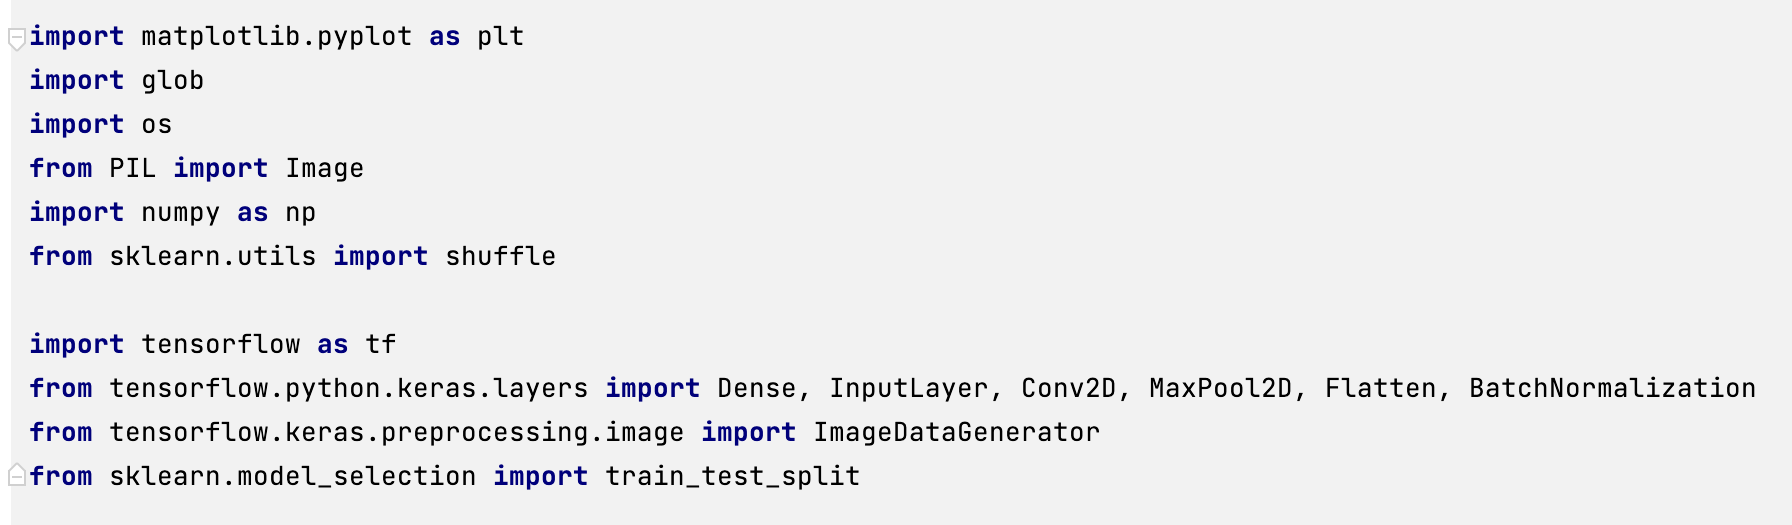
\includegraphics[width=10cm]{ESP32/Imports}
		\caption{Important Libraries} \label{fig:Imports}
		%{\footnotesize \textbf{Reference:} \cite{Network2020}}
	\end{center}
\end{figure}

For loading, initializing, and using \ac{nn}, a wrapper class will be required which also encapsulates the \ac{tfl} components. The actual code of \ac{tfl} that is tflite-lib will be needed to be adapted as per the ESP-IDF environment. Other than these, three files CMakeLists, sdkconfig, and partitions.csv are important. CMakeLists controls the details of the compiler for all components. The file sdkconfig has all compiler-specific settings for ESP32. The partitions.csv file has a user-defined partitioning of flash memory. The methods used in the wrapper class are shown in the following figure \ref{fig:WrapperClass}. \cite{Mueller:2022Part3}

\begin{figure}  
	\begin{center}
		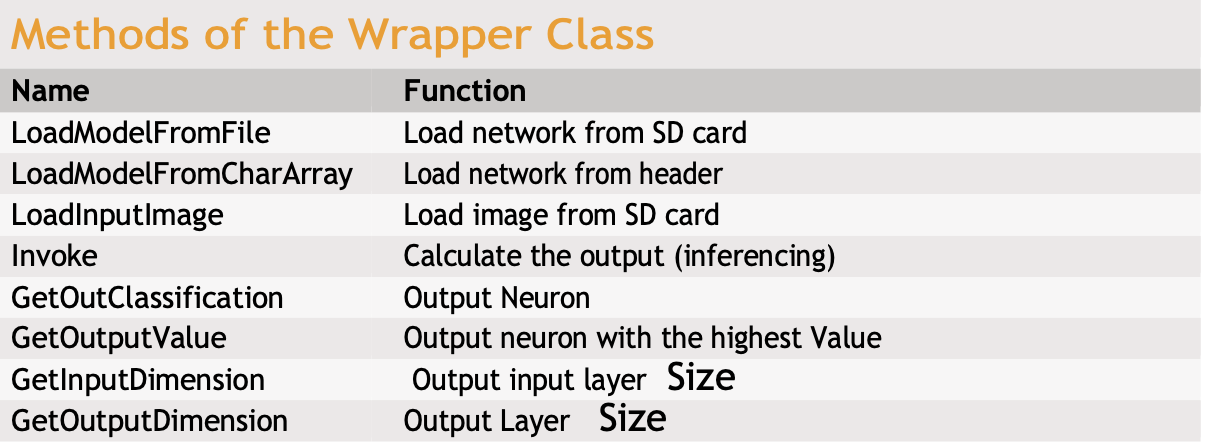
\includegraphics[width=10cm]{ESP32/WrapperClass}
		\caption{Methods in Wrapper Class} \label{fig:WrapperClass}
		{\footnotesize \textbf{Reference:} \cite{Mueller:2022Part3}}
	\end{center}
\end{figure}

\paragraph{Overview of the steps to use \ac{nn}}

A program needs to be created for using the neural network. This includes five steps namely: create an object of the wrapper class, load the model, load the image, calculate the \ac{nn} and read the results.

\paragraph{Working with the model}

Before loading the model, the SD card needs to be integrated with help of functions from the Helper library, the availability of PSRAM needs to be checked and an object from the needs to be created from CTfLiteClass to build a \ac{nn}.
Thereafter, the \ac{tfl} description of the \ac{nn} is loaded. The dynamic loading of a model from an SD card is preferred because of the memory management advantage. As a next step, the image is loaded from the SD card, and \ac{nn} is calculated. This can take some time. In the final step, the results can be read by selecting the ESP IDF Monitor Device option. The result could be saved on an SD card or displayed in a web application. As for now, we will consider the option of saving the results on an SD card.

%%%%%%%%%%%%%%%%%%%%%%%%%%%%%%%
\subsection{Hardware}

With regards to \ac{hw}, ESP32-CAM offers a lot of applications and is most commonly used on \ac{diy} projects. This is substantiated by the variety of modules and gadgets that can be added to this system. In addition to it, as has already been discussed low power applications, take huge advantage of these devices.  \cite{Babiuch:2019} 

Due to the wide variety of available sensors and applications aligned to this technology, it becomes imperative to describe how the final deliverable of the project will perform in terms of \ac{hw}. For this, a specific description of the key components of the system will be provided.

\bigskip

\addcontentsline{lot}{table}{\ac{hw} Deployment Description}

\begin{tabular}{llp{95mm}}
	\multicolumn{3}{l}{\large \textbf{\ac{hw} Deployment Description}}  \\ 
	\hline 
	& \textbf{SD Card Reader}  & This is one of the key points for this implementation, therefore it will be detailed in detail below. \\
	& \textbf{PSRAM} & The ESP32-CAM provides a processing power of 8 MByte in total, however, out of this value 4 MByte can be used for processing purposes.
	be used effectively. \\
	& \textbf{4 GByte Flash} & This is an external device that will be key to compliment both the \ac{sw} development for the model as well as the \ac{hw} limitations that come in addition to the device in question. \\
	& \textbf{ESP32-CAM-MB} & This is a special shield designed for easily transferring data from computer development to ESP32-CAM device. \\
	& \textbf{OV2640 camera} & This includes both the interface to plug the camera in the ESP32-CAM device and also the module itself, which was detailed in the Domain Knowledge of this same document.\\
	& \textbf{LED Flashlight} & This white LED incorporated in the board can be utilized as a flash for illuminating the meter, to improve the picture quality. \\
\end{tabular} \\

\bigskip

\subsubsection{SD Card implementation and uses}

Resuming the employment of both the "SD Card Reader" and the External extended memory device, these pieces of the system are key for complex implementations, such as \ac{cnn}. In principle, most of the basic projects that can be developed under \ac{iot} applications and some other fields can be easily mapped on the board's default firmware, and the capability will be enough. However, when it comes to more complex designs, with a large number of processes involved, it is better to have a robust infrastructure to support the analysis performed by the model. This project's specific implementation is designed to have over 100,000 nodes, which produces internal memory to be insufficient. In the \ac{sw} Deployment section of this same document is widely detailed how this module has to be included on the code to properly be recognized by the device. 

The purpose of this additional memory, from the SD Card, is to store sample images, in addition to the capability to dynamically load neural networks to the system, during the program's execution. \cite{Kontis:2017} This SD-Card has important details to consider, because, nothing can be so perfect. In this particular case, the limitation comes, ironically when using large storage drives (32/64 GB). This type of card can lead to a problem in the system, either when recognizing the SD Card, or when trying to access the images for the corresponding processing. This can be solved by using a 4GB (max) SD Card. \\

\subsubsection{ESP-CAM-MB}

To program the ESP32-CAM device it is required to meet certain \ac{hw} conditions, during the information transfer. 
The device is to be connected to a USB port in the computer, and through a USB-to-Serial converter, it can translate the information and program the microprocessor with the required functions. To avoid unnecessary wiring of the module, there is an available shield, which is specifically designed for this purpose on the ESP32-CAM. This shield has an integrated Micro-USB port, that will be the medium for the ESP32-CAM to communicate with the computer and vice-versa. To establish communication it is only required to plug the board into the shield since the pin-out is designed to match the exact distribution of the board. Internally the ESP-CAM-MB is designed to power up the device and enable the RX and TX pins of the device accordingly. 

\begin{figure}  
	\begin{center}
		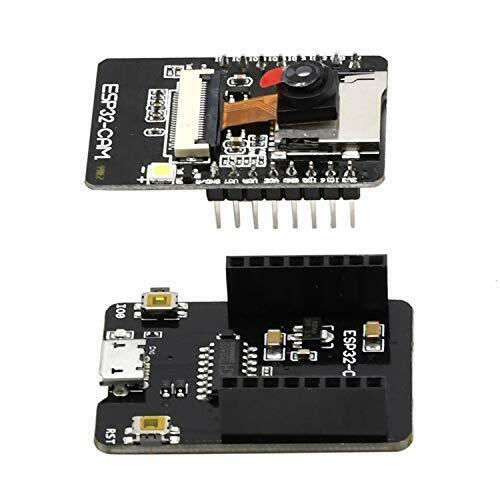
\includegraphics[width=12cm]{ESP32/Esp32CamMB}
		\caption{ESP32-CAM-MB connection plug to ESP32-CAM.} 
		\label{fig:ESP32-CAM-MB connection plug to ESP32-CAM.}
	\end{center}
\end{figure}	


Once both devices are paired, just as in the above picture is presented, the next required step is to plug a USB-micro-to-USB-A cable to connect to the \ac{pc} and upload the code.  

%%%%%%%%%%%%%%%%%%%%%%%%%%%%%%%
\subsection{Configuration}

Once the model is fitted and properly uploaded in the ESP32-CAM, the device will run under specific environmental conditions. In field application, the environment and conditions for the project to properly perform need to be very clearly set. The first thing is to understand the surroundings where the module is placed. In this application, the ESP32-CAM will be placed in front of a printed number (taken from a real meter). The device will be connected to the Computer directly; this is possible with the already-explained Mother Board shield. This will power the device during operation, and will also link the responses for the user, among other important calibration parameters for image capturing. 

\begin{figure}  
	\begin{center}
		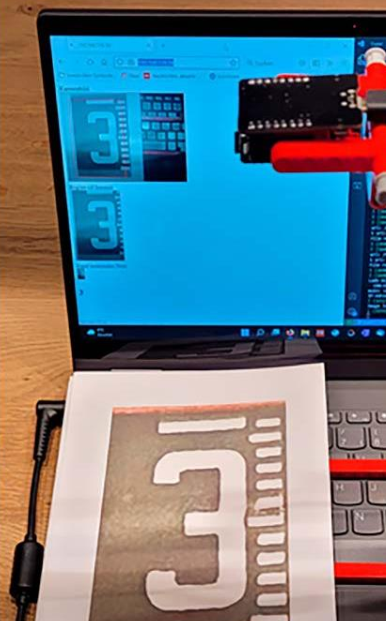
\includegraphics[width=12cm]{ESP32/ESP32CAMField}
		\caption{ESP32-CAM field application.} 
		\label{fig:ESP32-CAM field application.}
	\end{center}
\end{figure}	


The alignment is one of the key items to consider for precise image capturing, this means the correct orientation of the image. In the presented application this feature is not automatically solved by the program. However, adequate conditions are developed to achieve it. With the help of user input and an HTTP server (website), the alignment can be performed for each digit. The website is set so that it updates itself every 2 seconds, this will allow quick response and optimization of the results. Regarding web server details, it is accessed via its IP address. To make it easy for the user, this information will be displayed in the\ac{vscode} monitoring interface.\\

Sample images can be found under the code section in the \href{https://github.com/jomjol/ctmake-KI-ESP32-Teil2}{existing GitHub project}. Testing Images will be stored in a Word file (SampleImages.docx) in the folder named: "HWTest" for its simple printout and usage for future testing. After the image is properly set for alignment, by user input, in the same simple HTTP server to display the captured images, the output from the \ac{cnn} will also be displayed to the user as a resulting number.

%%%%%%%%%%%%%%%%%%%%%%%%%%%%%%%
\subsection{Tests}
It is clear that after all the previous steps, some parameters need to be defined for the project functionality. This subsection's objective is to present the result from the implementation on two fronts; \ac{hw} and \ac{sw}. It is important to specify this feature to understand how the system will be under corroboration in the coming steps.

%%%%%%%%%%%%%%%%%%%%%%%%%%%%%%%

\subsubsection{General Things to Consider during Deployment Testing}

The reliability of the neural network to recognize the digit increases with the increase in the training data. The neural network learns to abstract to the general rule and recognizes various aspects in the image such as contrast, brightness and other factors. For instance, if only one image per digit is used in the training of the data. And coincidentally, the image of the digit 1 is taken in a brighter setting (With better background light). Now when we train our neural network with this data, all the other digits might be recognized excellently but the other digits other than 1 can be recognized again and again. When we take a closer analysis, we can notice that this occurs whenever the background light is better. In this case our neural network did not recognize the digit 1 at all, but instead it recognizes the state of “brighter image”. To avoid such issues, it advised to have more training data with different properties of an image, such as varying brightness, position of the digits, different environments, and other factors \cite{Mueller:2022Part2}.

The raw images captured using the OV2640 camera module are of different sizes, it generally offers more resolution than what is actually needed for the neural computation. For the neural network to operate efficiently, a uniform input data variable must be provided. Generally, the size of the image directly influences the training speed of the neural network. With smaller image size, the training and recognition of the data is faster. On the other hand, there is a loss of information if the size of the image becomes too small. It is advisable to keep the images in a size, which is sufficient for the neural network to automatically recognize it \cite{Mueller:2022Part2,Schmidt:2019}.

%%%%%%%%%%%%%%%%%%%%%%%%%%%%%%%
\subsubsection{Software Behavior Results}

The following figure  gives an overview of the activities which are required for successfully completing the project.

\begin{figure}  
	\begin{center}
		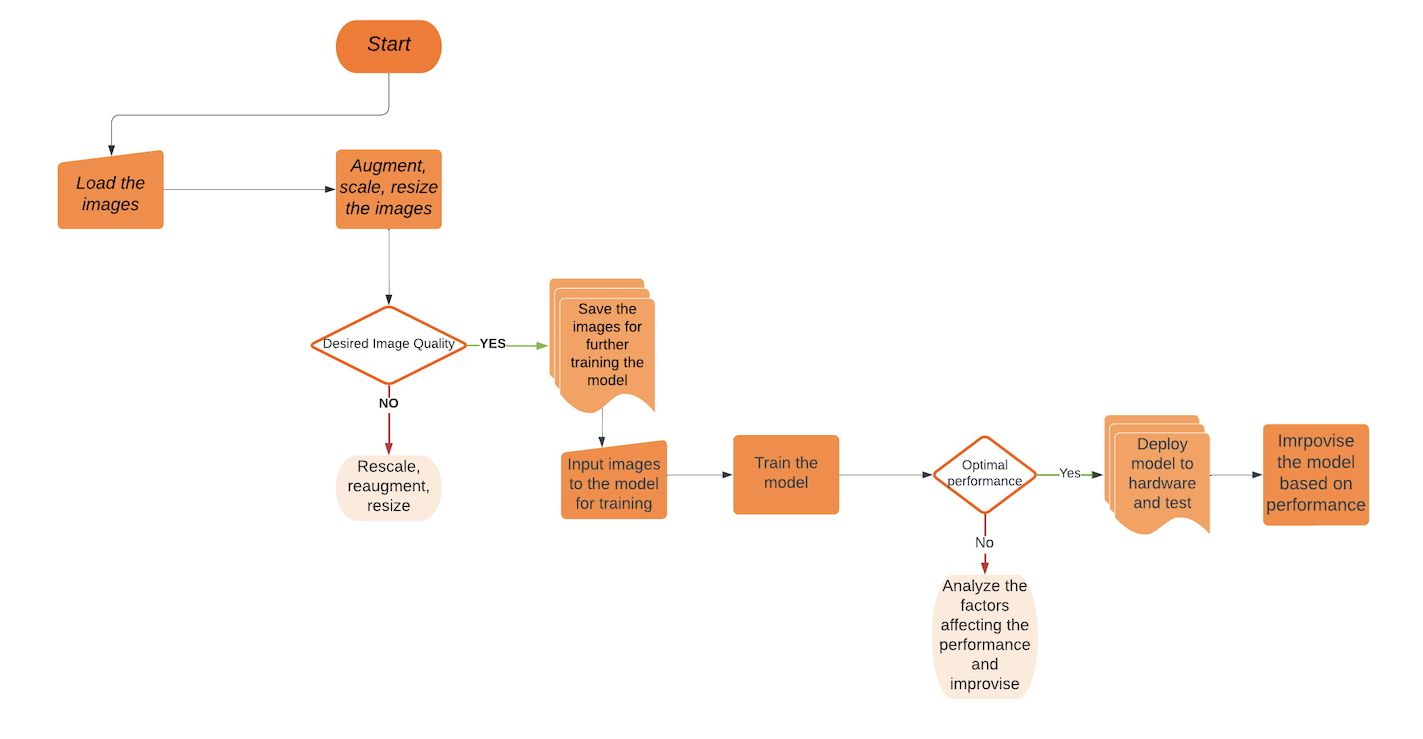
\includegraphics[width=15cm]{ESP32/SWFlowchart}
		\caption{Software flowchart} \label{fig:SWflowchart}
		%{\footnotesize \textbf{Reference:} \cite{Mueller:2022Part3}}
	\end{center}
\end{figure}

\paragraph{Software Tests}

After creating Python programs for loading and processing images, it should be tested that the intended results are achieved. Also, after fitting the model, the performnace of the \ac{cnn} needs to be checked that whether it is returning the desired results or not. Moreover, some negative test scenarios should be tested with the help of special characters and alphabets.

%%%%%%%%%%%%%%%%%%%%%%%%%%%%%%%
\subsubsection{Hardware Behavior Results}
Once code is implemented in the ESP32-CAM module, the system is capable of identifying and providing a digital response with the corresponding number. 

<Here the report will include images of the real project implementation> 

%%%%%%%%%%%%%%%%%%%%%%%%%%%%%%%

\section{Monitoring}
When the developers decide to modify the data set or add fresh training data, we monitor the model's behavior to observe and record it. Or whenever due to environment changes a data base suffers modifications, it is called: Monitoring. The data set for this project is mostly unchanged because it just includes digits and their many variations. In order to ensure that the model is robust enough since its first development, the TensorFlow library's ImageDataGenerator module is used to create several versions. 

The goal of this stage is to ensure that the knowledge that has been extracted from the data is being used to make informed decisions and to improve the overall performance of the system. During this stage, the following activities are performed:

\begin{itemize}
	\item \textbf{Performance monitoring:} This involves keeping a close eye on the effectiveness of the model created to interpret the data from the meters in order to make sure they are producing precise and pertinent findings.
	\item \textbf{Maintenance:} This entails maintaining the models and the database with fresh data and ensuring their functionality. In this particular case, since the data base is "numbers" then this is a very unusual case to happen, since numbers are universal.
	\item \textbf{Evaluation:} Finding any odd or unexpected trends in the meter data, such as sudden spikes or dips in use, is a part of this process.
	\item \textbf{Feedback:} This involves setting up automated alerts or notifications to let consumers know when particular criteria are satisfied, such when the use reaches a specific threshold or when a leak is discovered.
	\item \textbf{Continuous improvement:} To enhance the performance of the models and the whole KDD process, this entails regularly monitoring the system and making the appropriate adjustments.
\end{itemize}

The KDD process may be enhanced over time by continuously monitoring the models and the data to spot any flaws, inconsistencies, or outliers in the data and giving the system's users useful insights that enable them to make better educated decisions.

%%%%%%%%%%%%%%%%%%%%%%%%%%%%%%%
